\documentclass[12pt, psamsfonts]{amsart}

%-------Packages---------
\usepackage{amssymb,amsfonts}
\usepackage[all,arc]{xy}
\usepackage{enumerate}
\usepackage{mathrsfs}
\usepackage{theoremref}
\usepackage{graphicx}
\usepackage[bookmarks]{hyperref}

%--------Theorem Environments--------
%theoremstyle{plain} --- default
\newtheorem{thm}{Theorem}[section]
\newtheorem{cor}[thm]{Corollary}
\newtheorem{prop}[thm]{Proposition}
\newtheorem{lem}[thm]{Lemma}
\newtheorem{conj}[thm]{Conjecture}
\newtheorem{quest}[thm]{Question}

\theoremstyle{definition}
\newtheorem{defn}[thm]{Definition}
\newtheorem{defns}[thm]{Definitions}
\newtheorem{con}[thm]{Construction}
\newtheorem{exmp}[thm]{Example}
\newtheorem{exmps}[thm]{Examples}
\newtheorem{notn}[thm]{Notation}
\newtheorem{notns}[thm]{Notations}
\newtheorem{addm}[thm]{Addendum}
\newtheorem*{exer}{Exercise}

\theoremstyle{remark}
\newtheorem{rem}[thm]{Remark}
\newtheorem{rems}[thm]{Remarks}
\newtheorem{warn}[thm]{Warning}
\newtheorem{sch}[thm]{Scholium}

\DeclareMathOperator{\Hom}{Hom}
\DeclareMathOperator{\Id}{Id}

\makeatletter
\let\c@equation\c@thm
\makeatother
\numberwithin{equation}{section}

\bibliographystyle{plain}

\begin{document}

\title{Math 611 Homework 2 (Due 9/11)}
\author{Hidenori Shinohara}
\maketitle

\begin{exer}{(Problem 1, Section 1.2)}
  Show that the free product $G * H$ of nontrivial groups $G$ and $H$ has trivial center, and that the only elements of $G * H$ of finite order are the conjugates of finite-order elements of $G$ and $H$.
\end{exer}

\begin{proof}
  Let $w \in G * H$ be given.
  Suppose $w$ is not the empty word.
  \begin{itemize}
    \item
      Suppose the leftmost element of $w$ is in $G$.
      Let $h \in H$ be given such that $h$ is not the identity element of $H$.
      \begin{itemize}
        \item
          Case 1: The rightmost element of $w$ is an element of $G$.
          Then $wh$ is just a concatenation, so $wh \ne hw$ because the leftmost element of $wh$ is in $G$ and the leftmost element of $hw$ is in $H$.
        \item
          Case 2: The rightmost element of $w$ is an element of $H$, but not $h^{-1}$.
          Let $h'$ denote the rightmost element of $w$ and $w'$ denote the remaining.
          Then $w = w'h'$, so $wh = w'(h'h)$.
          By the definition of a reduced word, the rightmost element of $w'$ is an element of $G$, so the concatenation of $w'$ and $h'h$ is exactly $wh$.
          The leftmost element of $wh$ is in $G$ and the leftmost element of $hw$ is in $H$, so $wh \ne hw$.
        \item
          Case 3: The rightmost element of $w$ is $h^{-1}$.
          Then the rightmost element of $w$ disappears in $wh$.
          In this case, the leftmost element of $w$ stays the same.
          Therefore, the leftmost element of $wh$ is in $G$ and the leftmost element of $hw$ is in $H$, so $wh \ne hw$.
      \end{itemize}
      In each case, $wh \ne hw$.
    \item
      Suppose that the leftmost element of $w$ is in $H$.
      Let $g \in G$ be given such that $g$ is not the identity element of $G$.
      Using the exact same logic as above, we can conclude that $wg \ne gw$.
  \end{itemize}
  Therefore, $w$ is not in the center of $G * H$, so $Z(G * H) = \{ e \}$ where $e$ denotes the empty word.

  Let $x$ be a finite-order element in $G$ or $H$.
  Let $n$ denote the order.
  Let $w \in G * H$.
  Then $(wxw^{-1})^n = wx^nw^{-1} = ww^{-1} = e$, so the conjugate of a finite order element in $G$ or $H$ is has finite order.

  We will show that every element of finite order in $G * H$ is a conjugate of a finite order element in $G$ or $H$.
  We will consider the length of a finite-order element.
  \begin{itemize}
    \item
      Let $w \in G * H$ be a nonempty word of even length.
      Since adjacent elements must be elements of different groups, the leftmost element of $w$ and rightmost element of $w$ are in different groups.
      In other words, $w^k$ has the length $k$ times the length of $w$.
      This implies that the order of $w$ is not finite.
    \item
      We will show that every reduced word of length $2k - 1$ is a conjugate of a finite order element in $G$ or $H$ for every $k \in \mathbb{N}$.
      Let $k = 1$.
      Then it is either just $g$ or $h$ where $g \in G$ or $h \in H$.
      In each case, it is clear that the order $g$ or $h$ itself is finite.
      Therefore, it is a conjugate of a finite order element by the empty word.

      Suppose that the claim is true for some $k \in \mathbb{N}$.
      We will consider a finite-order element of length $2k + 1$.
      Let $w$ denote a reduced word of length $2k + 1$.
      Suppose $w^n = e$ for some $n \in \mathbb{N}$.
      \begin{itemize}
        \item
          Case 1: The leftmost element of $w$ is in $G$.
          Then $w = gw'g'$ where $g, g'$ are in $G$ and $w'$ is a reduced word of length $2k - 1$.
          $g'$ must equal $g^{-1}$.
          Otherwise, the length of $w^m$ would equal $m \cdot (2k + 1) - m$, and it would never equal 0.
          Consider $g^{-1}wg = w'$.
          Since $(g^{-1}wg)^n = g^{-1}w^ng = g^{-1}g = e$, the order of $w'$ is finite.
          By the inductive hypothesis, $w'$ is a conjugate of a finite order element in $G$ or $H$.
          Since the length of $w'$ is odd and the end elements are in $H$, $w'$ must be a conjugate of a finite order element in $G$.
          In other words, $w' = axa^{-1}$ for some $a \in G * H$ and $x \in G$.
          Then $w = g(axa^{-1})g^{-1} = (ga)x(a^{-1}g^{-1}) = (ga)x(ga)^{-1}$.
          $ga$ is a reduced word because the leftmost element of $a$ is the same as the leftmost element of $w'$, which is in $H$.

          By induction, every reduced word of finite length whose leftmost element is in $G$ is a conjugate of a finite order element in $G$.
        \item
          Case 2: The leftmost element of $w$ is in $H$.
          By symmetry, every reduced word of finite length whose leftmost element in $H$ is a conjugate of a finite order element in $H$.
      \end{itemize}

      Therefore, the only elements of $G * H$ of finite order are the conjugates of finite-order elements of $G$ and $H$.
  \end{itemize}
\end{proof}

\begin{exer}{(Problem 4, Chapter 1.2)}
  Let $X \subset \mathbb{R}^3$ be the union of $n$ lines through the origin.
  Compute $\pi_1(\mathbb{R}^3 - X)$.
\end{exer}

\begin{proof}
  When $n = 1$, the space can be deformation retracted to $S^1$.
  Thus $\pi_1(\mathbb{R}^3 - X)$ is $\mathbb{Z}$ when $n = 1$.
  Suppose $n \geq 2$.

  \begin{figure}
    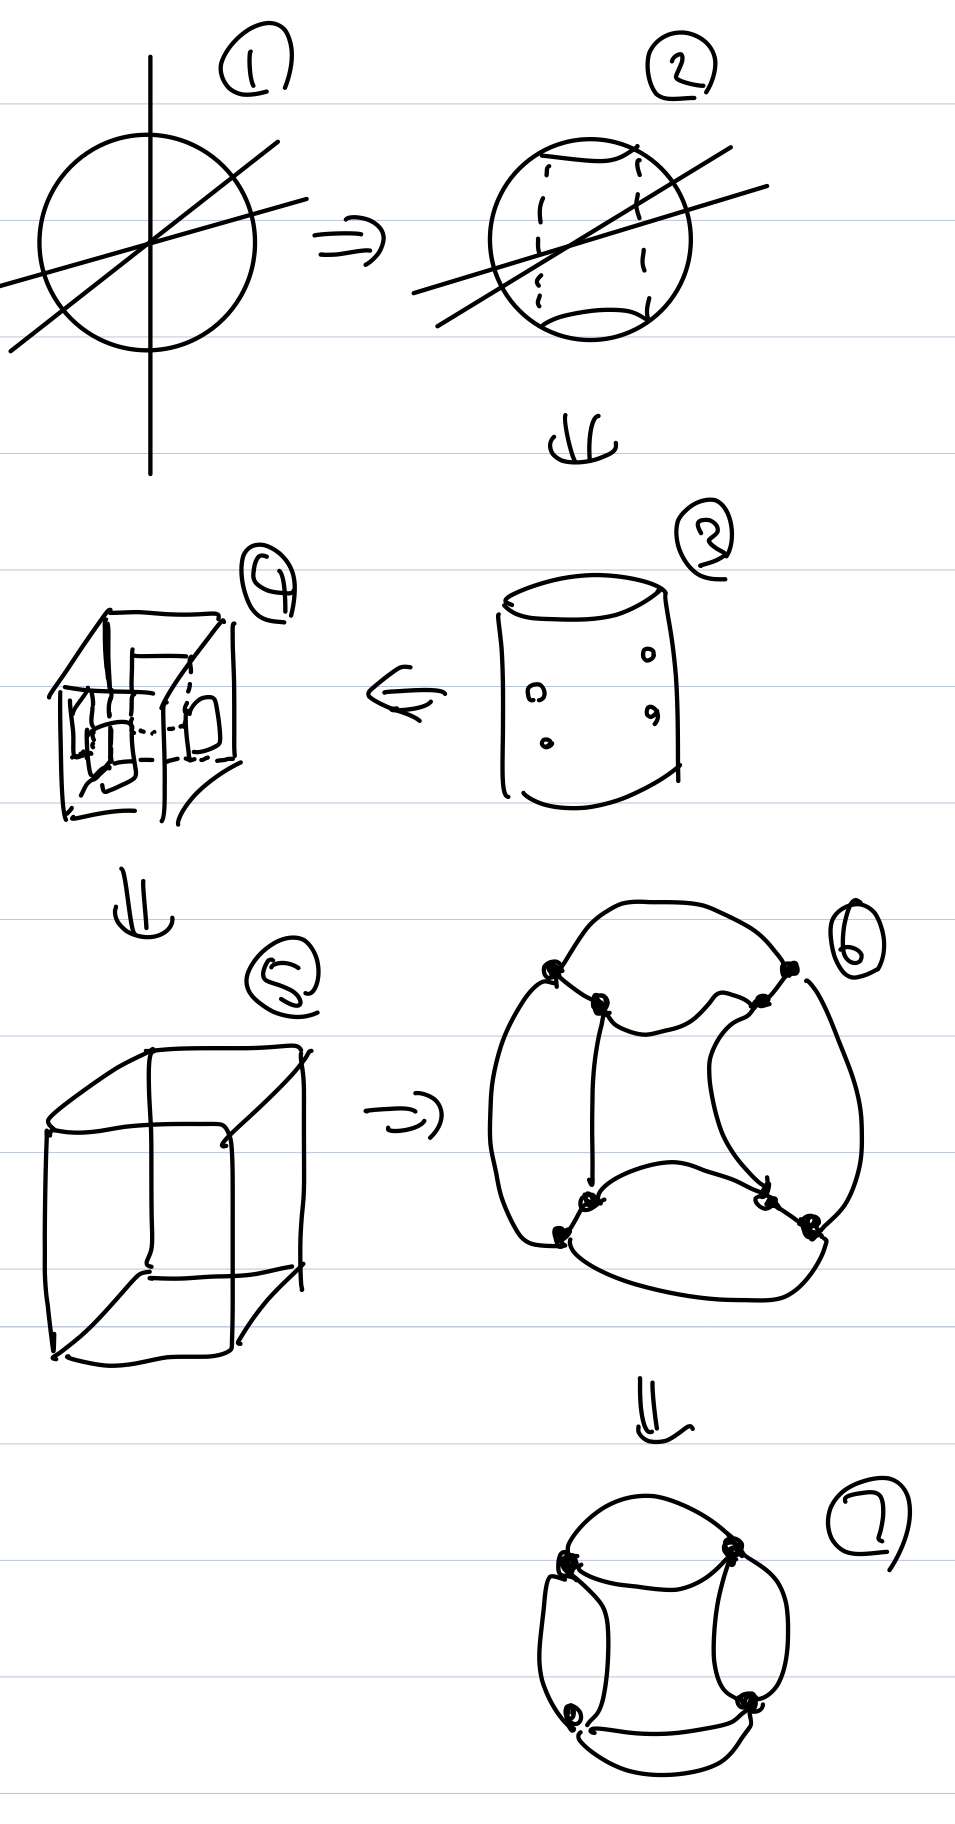
\includegraphics[width=.5\linewidth]{sphere_lines.jpeg}
      \caption{Transformation of $S^2$ with holes}
    \label{fig:transformation}
  \end{figure}
  Figure \ref{fig:transformation} shows how we will transform the space.
  \begin{itemize}
    \item
      $1$
      First, $\mathbb{R}^3$ can be deformation retracted to $S^2$.
    \item
      $1 \rightarrow 2$.
      Deformation retraction.
      Pick one of the lines and expand the hole.
    \item
      $2 \rightarrow 3$.
      Deformation retraction.
      Make the side thinner to create a tunnel with $2(n - 1)$ holes on the side.
      The number of holes on the side is always $2(n - 1)$ because there are $n - 1$ lines after picking the first line and each line creates two holes.
    \item
      $3 \rightarrow 4$.
      Deformation retraction.
      Place the $2(n - 1)$ holes evenly and expand each hole to create a ``slit".
    \item
      $4 \rightarrow 5$.
      Deformation retraction.
      Expand each hole so we are remained with a graph.
    \item
      $5 \rightarrow 6$.
      Homeomorphism.
    \item
      $6 \rightarrow 7$.
      Homotopy equivalence.
      Shrink each of the short edges so they turn into points.
      We end up with a graph with $2(n - 1)$ vertices $v_1, \cdots, v_{2(n - 1)}$ such that for each $v_i$, we draw two edges to the next vertex.
      In total, the graph has $4(n - 1)$ edges.
      In case that $2(n - 1) = 2$, we draw 2 (undirected) edges from $v_1$ to $v_2$ and 2 (undirected) edges from $v_2$ to $v_1$, so there are be 4 edges between $v_1$ and $v_2$.
  \end{itemize}

  We will calculate the fundamental group of such a space.
  Let $G_n$ denote such a graph for each $n$.
  We claim that the fundamental group of $G_n$ is $\mathbb{Z} * \cdots * \mathbb{Z}$ ($2n - 1$ times).
  \begin{itemize}
    \item
      Let $n = 2$.
      \begin{figure}
        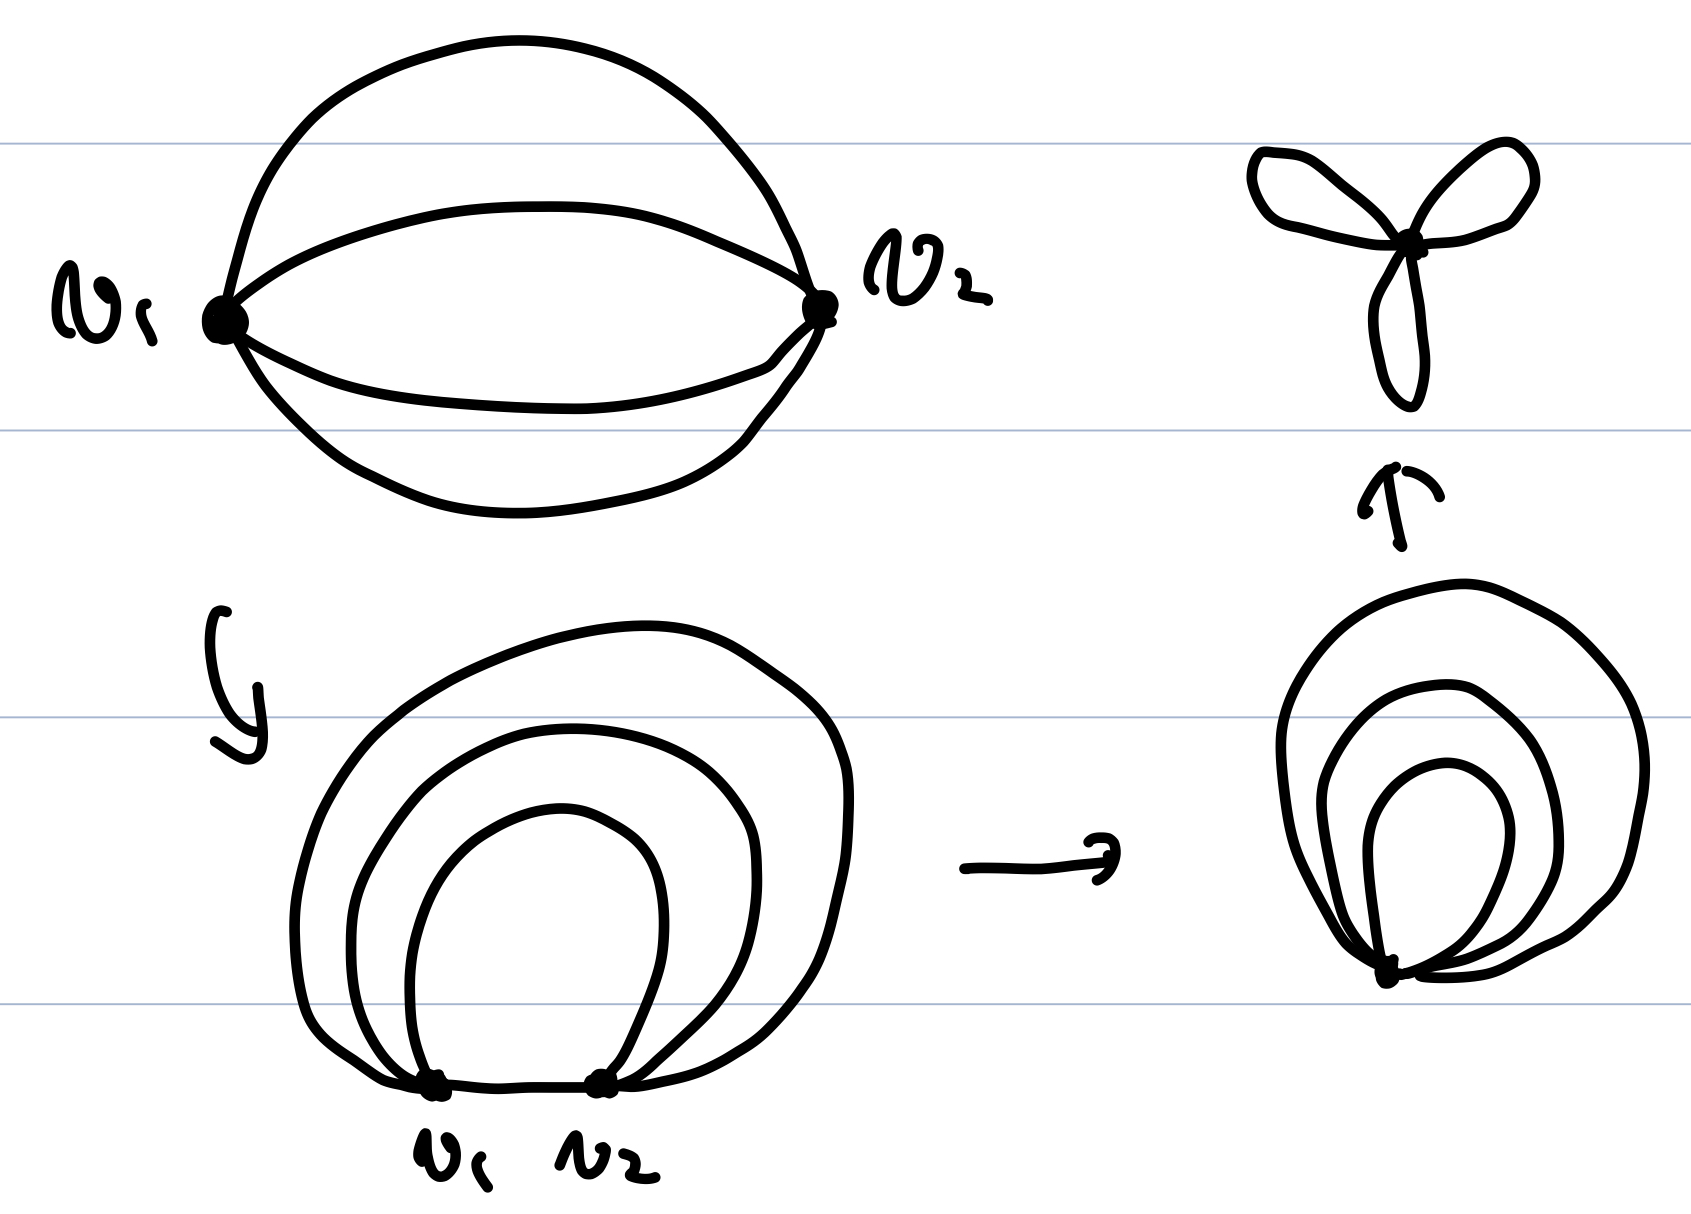
\includegraphics[width=.5\linewidth]{base_case.jpeg}
          \caption{Case 1: $n = 2$}
        \label{fig:n2}
      \end{figure}
      As in Figure \ref{fig:n2}, $G_2$ has the same fundamental group as a graph with one vertex and three loops.
      By Van Kampen's theorem, the fundamental group of two circles joined at a point is $\mathbb{Z} * \mathbb{Z}$ since the intersection is just a point.
      Similarly, the fundamental group of three circles joined at a point is $\mathbb{Z} * \mathbb{Z} * \mathbb{Z}$, which is $3 = 2n - 1$ times.
    \item
      Suppose the statement is true for some $n \geq 2$.
      Consider $G_{n + 1}$.
      As in Figure \ref{fig:ind}, $G_{n + 1}$ can be transformed into $G_{n}$ with two loops attached to one vertex without changing the fundamental group.
      \begin{figure}
        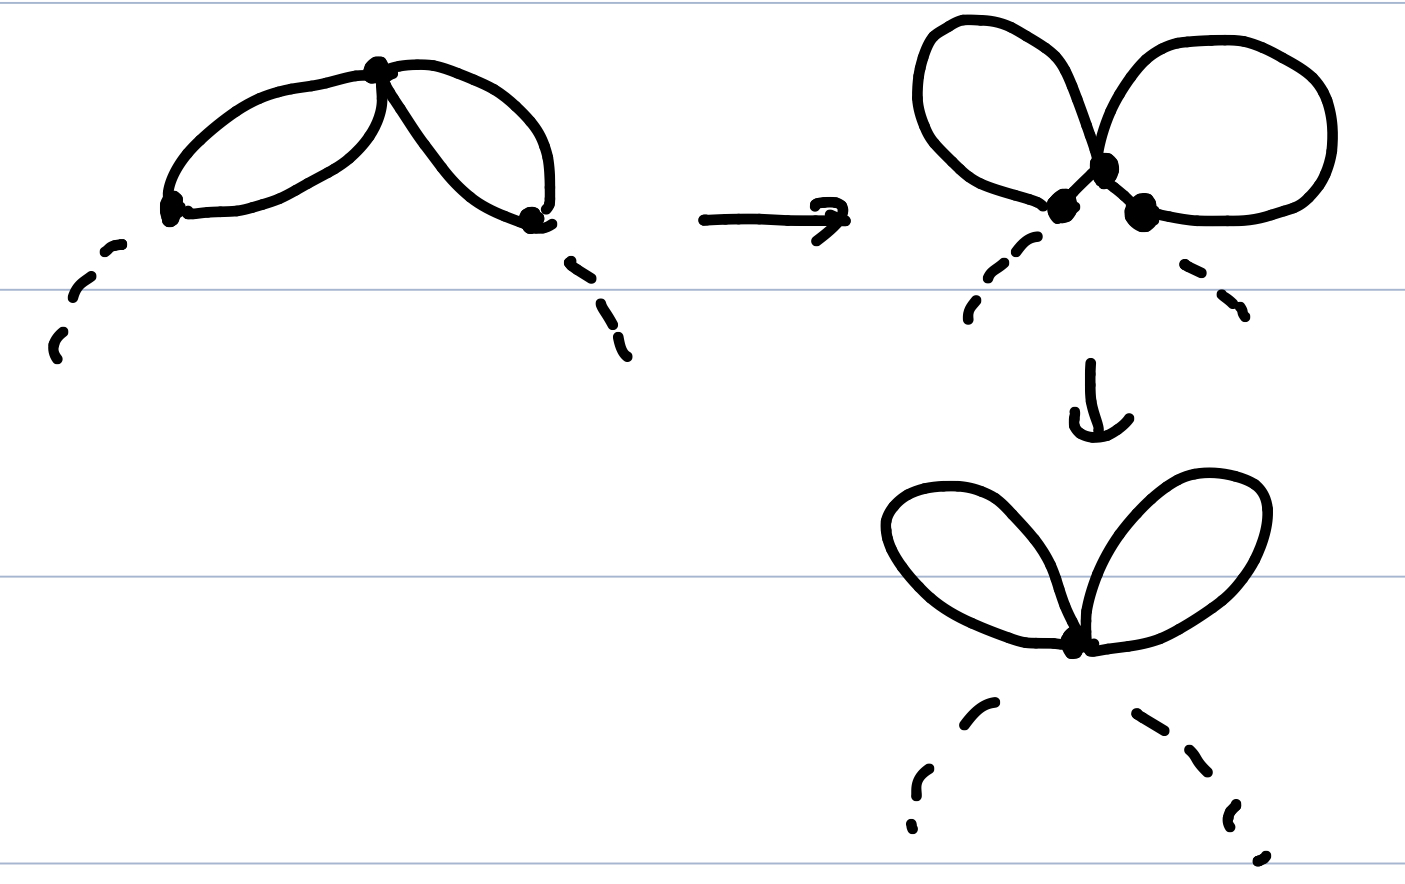
\includegraphics[width=.5\linewidth]{induction.jpeg}
          \caption{Inductive step}
        \label{fig:ind}
      \end{figure}
      By Van Kampen's theorem, the fundamental group of such a graph is $\pi_1(G_n) * \mathbb{Z} * \mathbb{Z}$.
      In other words, $\mathbb{Z} * \cdots * \mathbb{Z}$ ($2(n + 1) - 1$ times).
  \end{itemize}
\end{proof}

\begin{exer}{(Problem 8, Chapter 1.2)}
  Compute the fundamental group of the space obtained from two tori $S^1 \times S^1$ by identifying a circle $S^1 \times \{ x_0 \}$ in one torus with the corresponding circle $S^1 \times \{ x_0 \}$ in the other torus.
\end{exer}

\begin{proof}
  We consider a torus that is on another of the identical size such that they contact each other on the circle $S^1 \times \{ x_0 \}$ for some $x_0$.
  Let $T_1$ denote one of the tori and $T_2$ the other.
  Let $X = T_1 \cup T_2$.
  (Figure \ref{fig:tori})
  \begin{figure}
    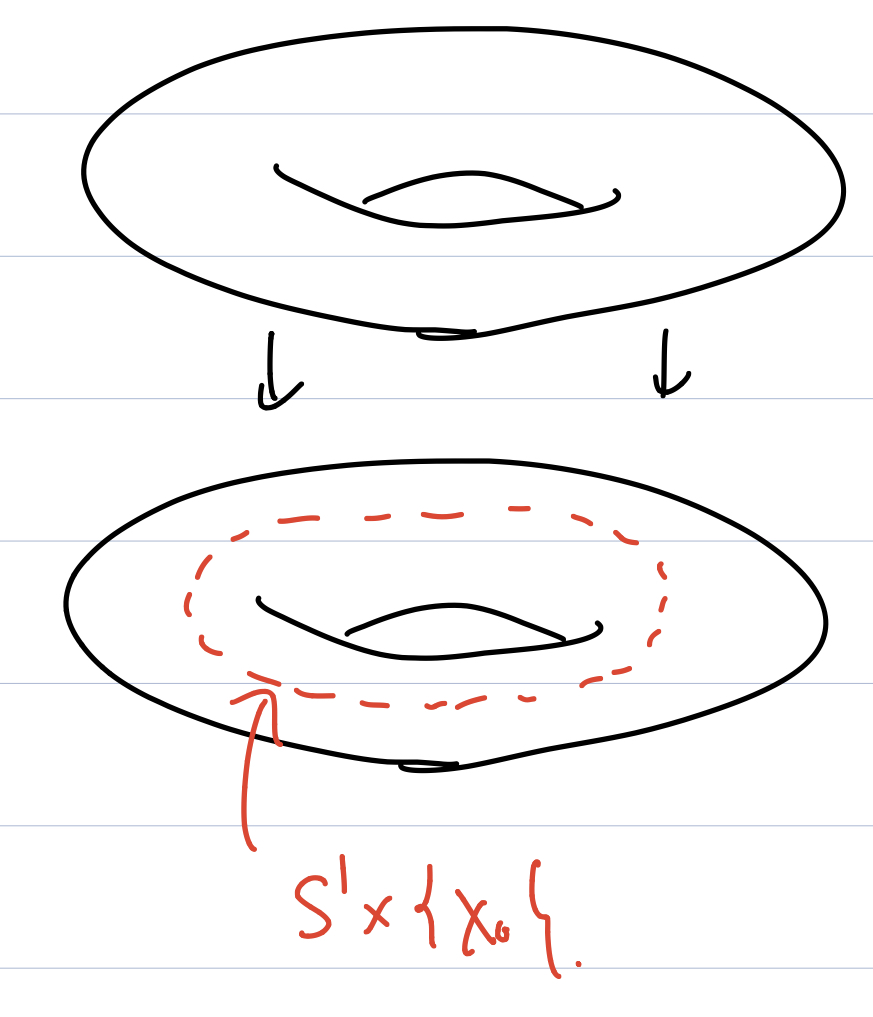
\includegraphics[width=.5\linewidth]{two-tori.jpeg}
      \caption{Two tori}
    \label{fig:tori}
  \end{figure}
  Each torus is path connected, and the intersection $S^1 \times \{ x_0 \}$ is also path connected.
  Let $p = (0, x_0)$.
  \begin{itemize}
    \item
      Let $w_1$ be a loop that goes around $S^1 \times \{ x_0 \}$ based at $p$ in $T_1$.
    \item
      Let $w_2$ be a loop that goes around $\{ 0 \} \times S^1$ based at $p$ in $T_1$.
    \item
      Let $w_3$ be a loop that goes around $S^1 \times \{ x_0 \}$ based at $p$ in $T_2$.
    \item
      Let $w_4$ be a loop that goes around $\{ 0 \} \times S^1$ based at $p$ in $T_2$.
  \end{itemize}
  Since $\pi_1(S^1 \times S^1) = \pi(S^1) \times \pi(S^1)$, $\pi_1(T_1, p) = \{ [w_1], [w_2] \mid [w_1][w_2] = [w_2][w_1]\}$ and $\pi_1(T_2, p) = \{ [w_3], [w_4] \mid [w_3][w_4] = [w_4][w_3]\}$.
  The fundamental group of the intersection $S^1 \times \{ 0 \}$ is the group generated by $[w_1]$, (or alternatively $[w_3]$).
  Let $i_1, i_2$ denote the injections from $\pi_1(T_1, p)$ and $\pi_1(T_2, p)$ into $\pi_1(T_1, p) * \pi_1(T_2, p)$, respectively.
  By Van Kampen's theorem, $\pi_1(T_1 \cup T_2, p) = \pi_1(T_1, p) * \pi_1(T_2, p) / \langle i_1([w_1])i_2([w_3])^{-1} \rangle$.
  To simplify the notations, let $a = [w_1], b = [w_2], c = [w_3], d = [w_4]$ and $N = \langle i_1(a)i_2(c) \rangle$.
  Then $\pi_1(T_1 \cup T_2, p) = \langle a, b \mid ab = ba \rangle * \langle c, d \mid cd = dc \rangle / N$.

  Let $(x_1, x_2, \cdots, x_n)N \in \pi_1(T_1 \cup T_2, p)$.
  For each $i$,
  \begin{itemize}
    \item
      Case 1: $x_i$ is an element of $\langle a, b \mid ab = ba \rangle$.
      Then $(x_i)N \in \langle a, b \mid ab = ba \rangle * \langle d \rangle / N$.
    \item
      Case 2: $x_i$ is an element of $\langle c, d \mid cd = dc \rangle$.
      By the commutativity, $x_i = c^id^j$ for some $i, j \in \mathbb{Z}$.
      Then $x_iN = (c^id^j)N = (c^iN)(d^jN) = (a^iN)(d^jN) = (a^i, d^j)N$, and $(a^i, d^j)N \in \langle a, b \mid ab = ba \rangle * \langle d \rangle / N$.
  \end{itemize}
  Therefore, each element in $\pi_1(T_1 \cup T_2, p)$ can be represented as cosets by words generated by $a, b, d$.
  Hence, $\pi_1(T_1 \cup T_2, p) = (\mathbb{Z} \times \mathbb{Z}) * \mathbb{Z}$.
\end{proof}

\end{document}


